\documentclass[pageno]{jpaper}
% \DeclareSymbolFont{letters}{OML}{ztmcm}{m}{it}
% \DeclareSymbolFontAlphabet{\mathnormal}{letters}

% Change to current semester and year, e.g.:
% \newcommand{\IWreport}{Spring 2020}
\newcommand{\IWreport}{Spring 2023}
\newcommand{\quotes}[1]{``#1''}
\newcommand{\lb}{\; | \;}
\newcommand{\tsteps}{\Mapsto_{\textrm{t}}}
\newcommand{\esteps}{\Mapsto_{\textrm{e}}}
\newcommand{\spacedot}{\; . \;}
\newcommand{\spaced}[1]{\; #1 \;}
\newcommand{\s}{\mathbb{S}}
\newcommand{\typrule}[3]{\frac{#1}{#2} \ \textbf{#3}}
\newcommand{\gamimp}{\Gamma \vdash}
\newcommand{\evalrule}[4]{\frac{#1}{#2} \ \boldsymbol{#3}_{\textbf{#4}}}
\newcommand{\env}{\mathtt{env}}
\newcommand{\prob}{\mathtt{prob} \ }
\newcommand{\angles}[1]{\langle #1 \rangle}
\newcommand{\parens}[1]{\llparenthesis #1 \rrparenthesis}
\newcommand{\evalenv}[1]{\langle \env, #1 \rangle}
\newcommand{\mt}[1]{\mathtt{#1}}
\newcommand{\rulename}[2]{$\boldsymbol{#1}_{\textbf{#2}}$}

\makeatletter
\def\verbatim@font{\linespread{1}\normalfont\ttfamily}
\makeatother

\widowpenalty=9999

\usepackage[normalem]{ulem}

\pagestyle{fancy}
\fancyhead[L]{IW Report}
\fancyhead[C]{\textbf{Implementing ProbaML}}
\fancyhead[R]{Spring 2023}

\begin{document}
\thispagestyle{empty}

\title{
  ProbaML: Implementation of a Functional Language Supporting Probabilistic Computation}

\author{Daniel Friedman\\\textbf{Adviser:} David Walker}

\date{}
\maketitle

\thispagestyle{empty}
\doublespacing
\begin{abstract}
\end{abstract}

\tableofcontents

\section{Introduction}
Functional programming languages have become increasingly popular in recent years due to their ability to reason about complex computations by using functions without side effects. This is especially important in probabilistic computations, which are inherently difficult to reason about due to the presence of randomness. In this paper, we present the design, operational semantics, and implementation of a custom functional language that supports probabilistic features such as sampling from distributions and computing expectations.

Probabilistic programming has gained significant attention in recent years due to its many applications in machine learning, robotics, and a variety of other fields. In addition, it is well suited for programs involving probabilistic computations and uncertainty. However, writing probabilistic programs can be challenging because they involve reasoning about random variables and their relationships. Functional programming paradigms have been shown to be well-suited for probabilistic programming because they provide a natural way to express computations involving randomness without side effects, enabling the programmer to write less error-prone code.

In this project, we explain the design and implementation of a custom functional language, \textbf{ProbaML}, that supports probabilistic features while utilizing the functional paradigm. The language includes support for expressing probability distributions and operations on them, as well as the ability to compute expectations. We believe that this language can be a useful tool for researchers and practitioners in the field of functional probabilistic programming.

Furthermore, the implementation of the language will provide a clear and concise example of how to build an interpreter from the ground up. This can be a valuable resource for students learning about functional programming concepts and language implementation. Overall, we believe that this project can contribute to the development of new and more efficient probabilistic programming languages and tools.

\section{Background and Related Work}

\subsection{Paper Formatting}
\label{section:formatting}

There has been a lot of work in the field of probabilistic programming, including that of functional probabilistic programming. As the uses of probabilistic data structures and other types of probabilistic analysis continue to grow, it becomes increasingly important to design languages and programming paradigms that make it easier to write bug-free code and reason about its correctness.

In Section~\ref{section:formatting}, we spoke about \cite{nicepaper,nicepaper2}.

\section{Problem Background and Related Work}
The following is a possible outline for your paper.

\section{Approach}
We rely on many of the features outlined in the cited paper that we will mention.

\section{Implementation}
The implementation of ProbaML is divided into several parts. First, we describe the abstract syntax for the language, its terms, expressions, and other components. Next, we describe the typing rules for ProbaML, and present an implementation of the type-checker in OCaml. We then proceed to describe the operational big-step semantics for the language, as well as the implementation of the evaluation in OCaml. We present two clients, a read-eval-print-loop and an evaluator to repeatedly compute a probabilistic sampling.
\subsection{Abstract Syntax}
\begin{figure}[hbt]
  \fbox{
    \parbox[c]{\textwidth}{
      \centering
      \begin{align*}
         & \textrm{type}              & A      & ::= A \rightarrow A \lb \square \ A \lb \text{real} \lb \text{int} \lb \text{bool} \\
         & \textrm{term}              & M,N    & ::= x \lb \lambda x:A.M \lb M M \lb \textrm{let } x = M \textrm{ in } N            \\
         &                            &        & \qquad \lb \textrm{prob } E \lb r                                                  \\
         & \textrm{expression}        & E      & ::= M \lb \textrm{sample } x \textrm{ from } M \textrm{ in } E \lb \s              \\
         & \textrm{value}             & V      & ::=  \lambda x:A.M \lb \textrm{prob } E \lb r                                      \\
         & \textrm{real number}       & r      &                                                                                    \\
         & \textrm{variable}          & x      &                                                                                    \\
         & \textrm{sampling sequence} & \omega & ::= r_1 r_2 \cdots r_i \cdots \quad \textrm{where $r_i \in (0.0, 1.0]$}            \\
         & \textrm{typing context}    & \Gamma & := \cdot \lb \Gamma \lb \Gamma, x:A
      \end{align*}
      \caption{Abstract syntax for ProbaML.}
      \label{fig:abstract_syntax}
    }}
\end{figure}
The above figure summarizes the types of terms in ProbaML. We begin with types, where the language supports the standard types, as well as a real number type and a $\text{prob } A$ type Note the distinction between \emph{terms} and \emph{expressions}.

\subsubsection{Implementation of the Abstract Syntax Tree}
\begin{Verbatim}[frame=single, baselinestretch=1, formatcom=\color{MidnightBlue}]
  (** The type of expressions in the abstract syntax tree (AST) **)
  type expr =
  (* Deterministic *)
  | Var of var                    // variables
  | Int of int                    // integers
  | Bool of bool                  // booleans
  | Float of float                // floating-pt numbers
  | Fun of var * typ * expr       // anonymous function definitions
  | Rec of var * var * expr * typ // recursive function definitions
  | Closure of var * var * expr * typ * env // function closures
  | App of expr * expr            // function application
  | Binop of bop * expr * expr    // binary-op expressions (+, -, *, <=)
  | Let of var * expr * expr      // let bindings
  | If of expr * expr * expr      // if-then-else expressions

  (* Probabilistic *)
  | Random                        // the uniform sampling expression S
  | Sample of var * expr * expr   // the 'sample from' binding
  | Prob of expr                  // probability distribution
  | AppProb of expr               // sampling from a distribution
  | Eif of expr * expr * expr     // eif-then-else expressions

  and env = expr Env.t // environment mapping variables to bindings
\end{Verbatim}

\subsection{Typing Rules}
As mentioned above, one of the key motivations for the creation of the language is that we can formalize its typing rules to ensure type safety. Since some expressions in ProbaML are probabilistic, it is especially significant to describe such judgments for probabilistic computations.

We begin by presenting the typing rules for deterministic terms, and then proceed to present those for probabilistic expressions.

We also briefly explain these rules, beginning with those of deterministic terms. See Figure~\ref{fig:typdeterm}.
\begin{itemize}
  \item The \textbf{Hyp}, \textbf{Lam}, \textbf{Fix}, \textbf{App}, and \textbf{If} rules are the standard typing rules for the typing axiom, function definition, recursive function definition, function application, and if statements respectively.
  \item The \textbf{Real} rule indicates the type of real numbers, $r$, in the language.
\end{itemize}
\begin{figure}[hbt]
  \fbox{
    \parbox[c]{0.98\textwidth}{
      \centering
      \setlength{\jot}{16pt}
      \begin{gather*}
        \typrule{}{\Gamma,x:A \vdash x:A}{Hyp} \quad \typrule{\Gamma,x:A \vdash M:B}{\Gamma \vdash \lambda x:A \; . \; M:A \rightarrow B}{Lam} \quad \typrule{\Gamma \vdash M_1:A \rightarrow B \quad \Gamma \vdash M_2:A}{\Gamma \vdash M_1 \ M_2 : B}{App}
        \\ \typrule{\Gamma, x:A \vdash M:A}{\Gamma \vdash \textrm{fix } x:A \; . \; M:A}{Fix} \quad \typrule{}{\Gamma \vdash r:\textrm{real}}{Real} \quad \typrule{\gamimp M : \textrm{bool} \quad \gamimp V_1:A \quad \gamimp V_2:A}{\gamimp \textrm{if } M \textrm{ then } V_1 \textrm{ else } V_2 : A}{If} \\
        \typrule{\gamimp V:B \quad \Gamma, x:B \vdash M:A}{\gamimp \textrm{let } x=V \textrm{ in } M:A}{Let}
      \end{gather*}
      \caption{Typing judgments for deterministic terms in ProbaML.}
      \label{fig:typdeterm}
    }}
\end{figure}
When discussing typing rules for probabilistic expressions, for a given typing environment $\Gamma$ type $A$, and computation $E$ we use the syntax $\Gamma \vdash E \gg A$ if $E$ \textit{computes} to a value of type $A$. Since $E$ is probabilistic, it need not yield the same value after it is computed every time the program is run. What is guaranteed, however, is that when the expression does compute to a specific value, that value will have type $A$. See Figure~\ref{fig:typprob}.

We briefly explain the typing rules incorporating probabilistic expressions.
\begin{itemize}
  \item The \textbf{Samp} rule states that $\mathbb{S}$ always computes to a value of type $r$ (a real number) in any context.
  \item The \textbf{Term} rule states that any term of type $A$ also computes to a value of type $A$. In other words, it is possible to transform a deterministic value into a degenerate probability distribution, and the value drawn from this distribution will always compute to a value of type $A$.
  \item The \textbf{Prob} rule is the intro rule for the \emph{prob} constructor. If $E$ computes to a value of type $A$, it creates a probability distribution, which now has type $\square \ A$.
  \item The \textbf{Bind} rule for expressions is the corresponding probabilistic term for the deterministic \emph{let} rule. It binds the variable $x$ to a sample from the probability distribution $M$ in the expression $E$.
  \item The \textbf{Unprob} rule allows for a shorter syntax to draw a single value from a probability distribution $M$. It takes a probability distribution as input and outputs a sample of type $A$ from that distribution.
  \item The \textbf{Eif} checks if $M$ is of type \emph{bool} and $E_1, E_2$ are probability distributions, and if so, draws a sample from either $E_1$ or $E_2$ which computes to a value of type $A$.
\end{itemize}

\begin{figure}[hbt]
  \fbox{
    \parbox[c]{0.98\textwidth}{
      \centering
      \setlength{\jot}{16pt}
      \begin{gather*}
        \typrule{}{\Gamma \vdash \mathbb{S} \gg r}{Samp}
        \quad \typrule{\Gamma \vdash M : A}{\Gamma \vdash M \gg A}{Term}
        \quad \typrule{\gamimp E \gg A}{\gamimp \textrm{prob } E : \square \ A}{Prob} \\
        \typrule{\gamimp M:\square \ A \quad \Gamma, x:A \vdash E \gg B}{\gamimp \textrm{sample } x \textrm{ from } M \textrm{ in } E \gg B }{Bind} \quad \typrule{\gamimp M:\square \ A}{\gamimp \textrm{unprob } M \gg A}{Unprob} \\
        \typrule{\gamimp M : \textrm{bool} \quad \gamimp E_1:\square \ A \quad \gamimp E_2:\square \ A}{\gamimp \textrm{eif } M \textrm{ then } E_1 \textrm{ else } E_2 \gg A}{Eif}
      \end{gather*}
      \caption{Typing judgments for probabilistic expressions in ProbaML.}
      \label{fig:typprob}
    }}
\end{figure}

\subsection{Operational Semantics}
We proceed to describe the big-step operational semantics of ProbaML. We first consider operational semantics for deterministic terms, and then extend the semantics with rules for probabilistic expressions. See Figure~\ref{fig:evaldeterm}.

We begin by explaining the rules for deterministic terms. We use the notation $M \tsteps N$ if $M$ big-steps to $N$ in a deterministic manner (there are no random terms in any of these kinds of expressions).
\subsubsection{Environment Model for Evaluation}
We use the environment model to evaluate expressions in ProbaML. In order to evaluate a term/expression, an \emph{environment} is required, which bounds a set of variables to their associated values. Non-function variables are evaluated and bound to their associated values. Function variables are evaluated and bound to their associated \emph{closures}, which is the function expression along with its defining environment. This defining environment is then used when evaluating a function application.

We begin by explaining some notation.
\begin{itemize}
  \item We use $\evalenv{E} \tsteps V$ to mean that the term $E$ evaluated in the environment $\mt{env}$ big-steps to a value $V$.
  \item $\env[x \rightarrow V]$ refers to the environment $\env$, \emph{extended} with one additional variable $x$ bound to value $V$.
  \item $\parens{\lambda x:A.M, \mt{def\_env}}$ refers to the \emph{closure} containing a function $\lambda x:A.M$ and its defining environment $\mt{def\_env}$.
\end{itemize}

We now explain the deterministic evaluation rules presented in Figure~\ref{fig:evaldeterm}.

\begin{itemize}
  \item The \rulename{T}{Hyp} rule defines environment extensions. It states that a variable $x$ evaluated in any environment extended with a binding of $x$ always evaluated to $V$, the value bound to $x$ in that environment.
  \item The \rulename{T}{Fun} rule is the anonymous function definition rule. It states that a function with environment $\env$ evaluates to a closure of the same function along with its \emph{defining environment}, $\mt{def\_env}$.
  \item The \rulename{T}{Fix} rule is the recursive function definition rule. It states that a recursive function named $f_{\textrm{name}}$ with environment $\env$ evaluates to the closure of the same function along with its defining environment.
  \item The \rulename{T}{App} rule is the function application rule. It states that if $M_1$ in environment $\env$ evaluates to a closure with function $\lambda x$ and defining environment $\mt{def\_env}$, $N$ in environment $\env$ evaluates to $V_1$, and extending the defining environment $\mt{def\_env}$ with $x$ bound to $V_1$ evaluates to $V_2$, then the function application of $N$ applies to $M_1$ in environment $\env$ evaluates to $V_2$.
  \item The \rulename{T}{AppRec} rule is the recursive function application rule. It states that (using environment $\env$) if $M_1$ evaluates to a closure for a recursive function, $N$ evaluates to a value $V_1$, and if $E_2$ evaluates to $V_2$ in an environment where extending the defining environment $\mt{def\_env}$ of the recursive function with $x$ bound to $V_1$ and the recursive function name $f_{\textrm{name}}$ bound to its closure, then the function application of $N$ applies to $M_1$ in environment $\env$ evaluates to $V_2$.
  \item The \rulename{T}{Let} rule is the let binding rule. It states that if (in environment $\env$) $E_1$ evaluates to $V_1$ and $M_2$ evaluates to $V_2$ in an environment where $\env$ is extended with the binding $x$ to $V_1$, then $\mt{let} \ x=M_1 \ \mt{in} \ M_2$ evaluates to $V_2$.
  \item The \rulename{T}{IfTrue} rule is the rule for if statements whose guard evaluates to $\mt{true}$.
  \item The \rulename{T}{IfFalse} rule is the rule for if statements whose guard evaluates to $\mt{false}$.
\end{itemize}

\begin{figure}[hbt]
  \fbox{
    \parbox[c]{0.98\textwidth}{
      \centering
      \setlength{\jot}{16pt}
      \begin{gather*}
        \evalrule{}{\angles{\env[x \rightarrow V], x} \tsteps V}{T}{Hyp} \\
        \evalrule{}{\langle \env, \lambda x:A.M \rangle \tsteps \parens{\mathtt{\lambda x:A.M, def\_env}}}{T}{Fun} \\
        \evalrule{}{\langle \env, \mathtt{fix} \ f_{\textrm{name}}:A \; . \; M \rangle \tsteps \parens{\mathtt{fix} \ f_{\textrm{name}}:A \; . \; M, \mathtt{def\_env}}}{T}{Fun} \\
        \evalrule{}{\angles{\env, \mathtt{fix} \ x:A.M} \tsteps \parens{\mathtt{fix} \ x:A.M , \mathtt{def\_env}}}{T}{Fix} \\
        \evalrule{\langle \env, M_1 \rangle \tsteps \llparenthesis \lambda x:A \spacedot M_2, \mathtt{def\_env} \rrparenthesis \quad \langle \env, N \rangle \tsteps V_1 \quad \angles{\mathtt{def\_env}[x \rightarrow V_1], M_2} \tsteps V_2}{\langle \env, M_1 \; N \rangle \tsteps V_2}{T}{App} \\
        \evalrule{\langle \env, M_1 \rangle \tsteps W \quad \langle \env, N \rangle \tsteps V_1 \quad \angles{\mathtt{def\_env}[x \rightarrow V_1, \mathtt{fname} \ \rightarrow W], M_2} \tsteps V_2}{\evalenv{M_1 \; N} \tsteps V_2}{T}{AppRec} \\[-14pt]
        \emph{where } W = \parens{\mathtt{fix} \ x:A.M, \mathtt{def\_env}} \\
        \evalrule{\langle \env, M_1 \rangle \tsteps V_1 \quad \langle \env[x \rightarrow V_1], M_2 \rangle \tsteps V_2}{\langle \env, \textrm{let } x = M_1 \textrm{ in } M_2 \rangle \tsteps V_2}{T}{Let} \\
        \evalrule{\evalenv{M} \tsteps \mathtt{true} \quad \evalenv{N_1} \tsteps V}{\evalenv{\mathtt{if} \ M \ \mathtt{then} \ N_1 \ \mathtt{else} \ N_2} \tsteps V}{T}{IfTrue} \\
        \evalrule{\evalenv{M} \tsteps \mathtt{false} \quad \evalenv{N_2} \tsteps V}{\evalenv{\mathtt{if} \ M \ \mathtt{then} \ N_1 \ \mathtt{else} \ N_2} \tsteps V}{T}{IfFalse}
      \end{gather*}
      \caption{Operational semantics for deterministic terms in ProbaML.}
      \label{fig:evaldeterm}
    }}
\end{figure}

\subsubsection{Deterministic Evaluation of Probabilistic Expressions}
We proceed to explain the evaluation rules for probabilistic terms in ProbaML. One of the motivations for ProbaML is to isolate the randomness and formalize the probabilistic computations in a deterministic manner. For this reason, we consider every expression to be evaluated with a \emph{sampling sequence}, an infinite list of randomly generated numbers $\omega=r_1 r_2 r_3 \cdots$. After an expression is evaluated, it consumes a finite amount of these numbers in order from $\omega$, and we call the remained of this infinite list $\omega'$
We represent the evaluation of probabilistic expressions as $\evalenv{E} @ \omega \esteps V \omega'$, meaning that a term $E$ in environment $\env$ with sampling sequence $\omega$ \emph{probabilistically steps} to a value $V$, consuming zero or more numbers from $\omega$ and returning $\omega'$. Note that $\evalenv{E} @ \omega \esteps V \omega'$ is deterministic. It is only when the sequence $\omega$ changes that the evaluation may produce a different result, but when $\omega$ is consistent, the result will always be the same.

We now explain the probabilistic evaluation rules presented in Figure~\ref{fig:evalproba}.

\begin{itemize}
  \item The \rulename{E}{Samp} rule is the random sampling rule. Given any environment $\env$ and number $r$ followed by a sequence $\omega$, $\mathbb{S}$ will consume and output the first number of that sequence, $r$, and return the rest of the sequence $\omega$.
  \item The \rulename{E}{Bind} is the let binding rule when drawing from probability distributions. It states that if (in some environment $\env$ and sampling sequence $\omega$) $E_1$ evaluates to some probability distribution $\mt{prob} \ E_2$ with remaining sampling sequence $\omega'$, $E_2$ computes to some value $V_1$, and $E_2$ computes to $V_2$ in the environment $\env$ with the binding $x$ to $V_1$, then $\mt{sample} \ x \ \mt{from} \ E_1 \ \mt{in} \ E_2$ with sampling sequence $\omega$ evaluates to $V_2$ along with the remaining sampling sequence $\omega'''$.
  \item The \rulename{E}{Unprob} rule is the rule for sampling a single value from a probability distribution. It states that if $E_1$ evaluates to some probability distribution $\prob E_2$ and $E_2$ computes to a value $V$, then $\mt{unprob} \ E_1$ returns this value $V$ along with the remaining sampling sequence.
  \item The \rulename{E}{IfTrue} rule is the if-statement rule for sampling from a probability distribution when the if-guard evaluates to $\mt{true}$. It states that if the guard evaluates to true and the first term evaluates to a probability distribution, and that distribution computes to a value when sampled, then $\mt{eif} \ M \ \mt{then} \ E_1 \ \mt{else} \ E_2$ evaluates to a sample drawn from probability distribution $E_2$.
  \item The \rulename{E}{IfFalse} rule is corresponding rule to the \rulename{E}{IfTrue} above, except when the if-guard evaluates to $\mt{false}$.
\end{itemize}

\begin{figure}[hbt]
  \fbox{
    \parbox[c]{0.98\textwidth}{
      \centering
      \setlength{\jot}{16pt}
      \begin{gather*}
        \evalrule{}{\langle \env, \mathbb{S} \rangle @ r \omega \esteps r @ \omega}{E}{Samp} \\
        \evalenv{E_1}@\omega \esteps \mt{prob} \ E_2 @ \omega' \\[-14pt]
        \evalrule{\evalenv{E_2} @ \omega' \esteps V_1 @ \omega'' \quad \langle \env[x \rightarrow V_1], E_2 \rangle @ \omega'' \esteps V_2 @ \omega'''}{\evalenv{\mt{sample} \ x \ \mt{from} \ E_1 \mt{in} \ E_2} @ \omega \esteps V_2 @ \omega'''}{E}{Bind} \\
        \evalrule{\evalenv{E_1}@\omega \tsteps \mt{prob} \ E_2 \quad \evalenv{E_2}@\omega \esteps V @ \omega'}{\evalenv{\mt{unprob} \ E_1} @ \omega \esteps V @ \omega''}{E}{Unprob} \\
        \evalenv{M}@\omega \esteps \mt{true} @ \omega' \\[-14pt]
        \evalrule{\evalenv{E_1} @ \omega' \esteps \prob E_3 @ \omega'' \quad \evalenv{E_3} @ \omega'' \esteps V @ \omega'''}{\evalenv{\mt{eif} \ M \ \mt{then} \ E_1 \ \mt{else} \ E_2} @ \omega \esteps V @ \omega'''}{E}{EifTrue} \\
        \evalenv{M}@\omega \esteps \mt{false} @ \omega' \\[-14pt]
        \evalrule{\evalenv{E_2} @ \omega' \esteps \prob E_3 @ \omega'' \quad \evalenv{E_3} @ \omega'' \esteps V @ \omega'''}{\evalenv{\mt{eif} \ M \ \mt{then} \ E_1 \ \mt{else} \ E_2 @ \omega \esteps V @ \omega'''}}{E}{EifFalse}
      \end{gather*}
      \caption{Operational semantics for probabilistic terms in ProbaML.}
      \label{fig:evalproba}
    }}
\end{figure}

\subsection{Implementation of Type Checker}
After completing the parsing and lexing, we implement the type checker for the abstract syntax tree using a recursive OCaml function \texttt{typeof}. First, we define a ProbaML type in the following OCaml data type, \texttt{typ}.

\begin{Verbatim}[frame=single, baselinestretch=1, formatcom=\color{MidnightBlue}]
  type typ =
  | TInt                   // A ProbaML int
  | TBool                  // A ProbaML bool
  | TReal                  // A ProbaML float
  | TProb of typ           // A ProbaML probability distribution type
  | TArrow of typ * typ    // A ProbaML arrow type
\end{Verbatim}

\begin{verbatim}
  let rec typeof (ctx : Context.t) (expr : expr) : typ = match expr with
    | Int _ -> TInt
    | Float _ -> TReal
    | Prob e -> TProb (typeof ctx e)
    | Closure (_, _, _, typ, _) -> typ
    | Var x -> Context.lookup ctx x
    | Let (x, e1, e2) -> let t' = typeof ctx e1 in
                         let ctx' = Context.extend ctx x t' in
                         typeof ctx' e2
    | AppProb e -> ( match typeof ctx e with
                   | TProb e' -> e'
                   | _ -> type_error Errors.proba_err )
    | App (e1, e2) -> ( match typeof ctx e1, typeof ctx e2 with
                      | TArrow (typ1, typ2), typ3 when typ1 = typ3 -> typ2
                      | _ -> type_error Errors.app_err )
    | Sample (x, e1, e2) -> ( match typeof ctx e1 with
                            | TProb t ->
                              let ctx' = Context.extend ctx x t in
                              typeof ctx' e2
                            | _ -> type_error Errors.bind_sample_err )
    ...
\end{verbatim}

\subsection{Implementation of Evaluation Relation}
\lipsum[1-2]

\newpage
\subsection{Examples of Probabilistic Computation in ProbaML}
We describe some examples defining probabilistic distributions and computations, along with their corresponding code.

\subsubsection{The Uniform Distribution}
\begin{figure}[hbt]
  \fbox{
    \parbox[c]{0.98\textwidth}{
      \centering
      \setlength{\jot}{10pt}
      \begin{align*}
        \mt{let} \textcolor{magenta}{\textit{ uniform}} = \  & \mt{fun} \ a \mt{:real \ -> \ fun} \ b \ \mt{:real \ -> } \\
        \mt{prob} \                                          & \mt{sample} \ x \ \mt{from \ prob} \ \s \ \mt{in}         \\
                                                             & a + x * (b - a)
      \end{align*}
      \caption{The Uniform Distribution in ProbaML.}
      \label{fig:uniform}
    }}
\end{figure}

\subsubsection{The Bernoulli Distribution}
\begin{figure}[hbt]
  \fbox{
    \parbox[c]{0.98\textwidth}{
      \centering
      \setlength{\jot}{10pt}
      \begin{align*}
        \mt{let} \textcolor{magenta}{\textit{ bernoulli}} = \  & \mt{fun} \ p \ \mt{:real \ ->}                    \\
        \mt{prob} \                                            & \mt{sample} \ x \ \mt{from \ prob} \ \s \ \mt{in} \\
                                                               & x \leq p
      \end{align*}
      \caption{The Bernoulli Distribution in ProbaML.}
      \label{fig:bernoulli}
    }}
\end{figure}

\subsection{The Exponential Distribution}
\begin{figure}[hbt]
  \fbox{
    \parbox[c]{0.98\textwidth}{
      \centering
      \setlength{\jot}{10pt}
      \begin{align*}
        \mt{let} \textcolor{magenta}{\textit{ exponential}} = \  & \mt{fun} \ \lambda \ \mt{:real \ -> }             \\
        \mt{prob} \                                              & \mt{sample} \ x \ \mt{from \ prob} \ \s \ \mt{in} \\
                                                                 & -1/\lambda * \log{x}
      \end{align*}
      \caption{The Exponential Distribution in ProbaML.}
      \label{fig:exponential}
    }}
\end{figure}


\subsection{The Geometric Distribution}
\begin{figure}[hbt]
  \fbox{
    \parbox[c]{0.98\textwidth}{
      \centering
      \setlength{\jot}{10pt}
      \begin{align*}
        \mt{let \ fix} \ \textcolor{magenta}{\textit{geometric}} = \  & \mt{fun} \ p \ \mt{:real \ ->}                                                                               \\
                                                                      & \mt{let} \ \textcolor{purple}{\textit{bernoulli}_{p}} = \textcolor{purple}{\textit{ bernoulli }} p \ \mt{in} \\
        \mt{prob} \                                                   & \mt{sample} \ b \ \mt{from} \ \textcolor{purple}{\textit{bernoulli}_{p}} \ \mt{ in}                          \\
                                                                      & \mt{eif} \ b \ \mt{then \ 0}                                                                                 \\
                                                                      & \mt{else \ sample} \ x \ \mt{from} \ \textcolor{magenta}{\textit{geometric}} \ \mt{in} \ 1+x
      \end{align*}
      \caption{The Geometric Distribution in ProbaML.}
      \label{fig:geometric}
    }}
\end{figure}

\subsubsection{The Gaussian Distribution}
\begin{figure}[hbt]
  \fbox{
    \parbox[c]{0.98\textwidth}{
      \centering
      \setlength{\jot}{10pt}
      \begin{align*}
        \mt{let} \textcolor{magenta}{\textit{ gaussian}} = \  & \mt{fun} \ m \mt{:real \ -> \ fun} \ \sigma \ \mt{:real \ -> } \\
        \mt{prob} \                                           & \mt{sample} \ u \ \mt{from \ prob} \ \s \ \mt{in}              \\
                                                              & \mt{sample} \ v \ \mt{from \ prob} \ \s \ \mt{in}              \\
                                                              & m + \sigma * \sqrt{-2.0 * \log u} * \cos (2.0 * \pi * v)
      \end{align*}
      \caption{The Gaussian Distribution in ProbaML.}
      \label{fig:gaussian}
    }}
\end{figure}

\subsection{REPL}

\section{Evaluation and Results}
\subsection{Graphing the Results and Jupyter Notebook}

\begin{figure}[hbt]
  \centering
  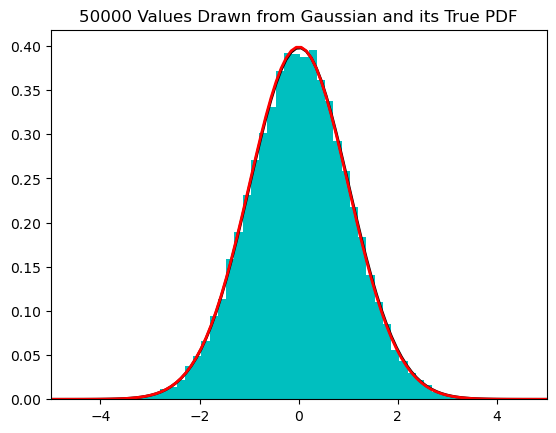
\includegraphics[scale=1]{gaussian.png}
  \caption{PDF of the Gaussian distribution overlaid with the distribution generated from ProbaML.}
\end{figure}

\begin{figure}[hbt]
  \centering
  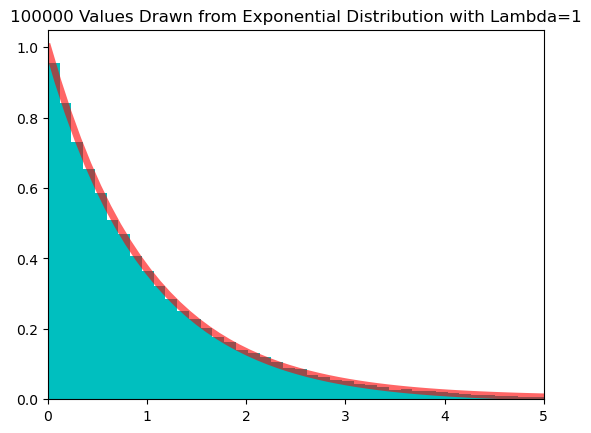
\includegraphics[scale=1]{exponential.png}
  \caption{PDF of the exponential distribution overlaid with the distribution generated from ProbaML.}
\end{figure}

\section{Conclusions}

\bstctlcite{bstctl:etal, bstctl:nodash, bstctl:simpurl}
\bibliographystyle{IEEEtranS}
\bibliography{references}

\end{document}